\chapter{Equations}
\section{Quadratic equations}
\begin{dfn}
A quadratic equation is an equation of the form
\begin{equation}
 \label{quad}
 ax^2 + bx + c = 0
\end{equation}
where \( a, b \) and \( c \) are constants and \( a \neq 0 \).
\end{dfn}

Let us draw a graph/picture \\
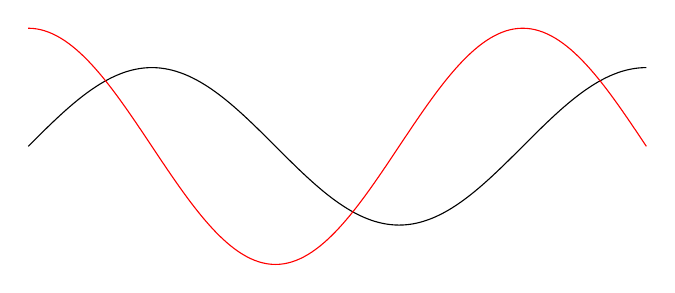
\begin{tikzpicture}[xscale=1.57]
\draw (0,0) sin (1,1) cos (2,0) sin (3,-1) cos (4,0) sin (5,1);
\draw[color=red] (0,1.5) cos (1,0) sin (2,-1.5) cos (3,0) sin (4,1.5) cos (5,0);
\end{tikzpicture}

Another picture:

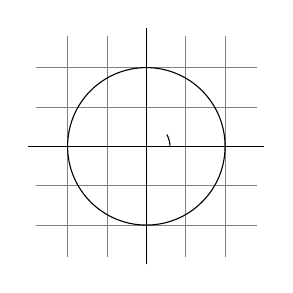
\begin{tikzpicture}
\draw[step=.5cm,gray,very thin] (-1.4,-1.4) grid (1.4,1.4);
\draw (-1.5,0) -- (1.5,0);
\draw (0,-1.5) -- (0,1.5);
\draw (0,0) circle [radius=1cm];
\draw (3mm,0mm) arc [start angle=0, end angle=30, radius=3mm];
\end{tikzpicture}
